\chapter{Umsetzung und Ablauf der Kalibrierung}

Der neu festgelegte Ablauf der Kalibrierung lässt sich in die zwei Schritte 
Einrichtung und Durchführung unterteilen. Die Einrichtung erfordert Kenntnisse
über die Funktionsweise des Kalibrierablaufs, muss aber nur einmalig pro Roboter
ausgeführt werden.

\section{Einrichtung der Kalibrierung}
\label{sec:Einrichtung der Kalibrierung}

Die Einrichtung der Kalibrierung kann vollständig in Simulation erfolgen und 
umfasst nur Änderungen der Dateien im Package \texttt{cob\_calibration\_config}. 


\subsection{Angeben der zu kalibrierenden Kameras und des Kalibrierobjekts}
\label{sub:Angeben der zu kalibrierenden Kameras}

Ein weiterer neuer Schritt bei der Einrichtung der Kalibrierung auf einem neuen
Roboter ist das Festlegen der zu kalibrierenden Kameras. Hierzu werden in der 
Datei \texttt{cameras.yaml} eine Referenzkamera und alle weiteren Kameras angegeben.
Dazu wird für jede Kamera der Name des Sensorkoordinatensystems, das
\ac{ROS}-Topic, auf dem die Bildinformationen verteilt werden und der Pfad zu den
Kalibrierungsdateien angegeben. Außerdem muss das eingesetzte Kalibrierungsmuster
angegeben werden. 

Diese Einstellungen waren bei dem ursprünglichen Kalibrierverfahren an mehreren 
Stellen verteilt, was das Anpassen an neue Roboter erschwert hat.
\subsection{Ausgangspunkt der Kalibrierung}
\label{sub:Ausgangspunkt der Kalibrierung}

Als
erster Schritt muss die neue Konfigurationsdatei \texttt{calibration\_seed.yaml} 
angelegt werden, in der eine Position des Kalibrierobjekts mittig im Sichtfeld
der Kameras in Gelenkwinkeln der Aktoren angegeben wird. Diese Position ist der Ausgangspunkt
der Kalibrierung und sollte genutzt werden, um den Endefektor des Roboters durch 
das Kalibrierobjekt zu ersetzen. Die angegebene Position wird als Anfangspunkt 
für die Suche der Samplepositionen verwendet.

\subsection{Berechnung der Samplepositionen}
\label{sub:Berechnung der Samplepositionen}
Die Samplepositionen werden automatisch berechnet. Dazu muss der Ausgangspunkt 
der Kalibrierung bekannt sein. Bei der Berechnung wird ein Bereich im Arbeitsraum
der zu kalibrierenden Aktorkette festgelegt. Danach werden für einzelne
Positionen in diesem Raum Berechnungen zur Sichtbarkeit und zur Erreichbarkeit 
der Positionen ausgeführt. Dazu wird mit einem allgemeinen Kameramodell, das nur
den Öffnungswinkel des Bildes benötigt und einem Modell der Bewegung der 
optischen Achse berechnet, ob die Position sichtbar ist. Im Anschluss daran wird
gegebenenfalls die inverse Kinematik des Torsos und des Arms berechnet. Die 
berechneten Gelenkwinkel werden in der Datei \texttt{calibration\_positions.yaml}
gespeichert. Die berechneten Positionen können anschließend durch Simulation
überprüft und manuell um weitere Positionen erweitert werden. Im Gegensatz zur 
bisherigen Kalibrierung lassen sich durch die neue Berechnung schneller
Gelenkwinkel für Roboter mit unterschiedlichen Arbeitsräumen festlegen. 

\subsection{Festlegung der Kinematischen Pfade}
\label{sub:Festlegung der Kinematischen Pfade}
Für jeden weiteren Schritt müssen Informationen, welche
kinematischen Ketten an der Kalibrierung beteiligt sind, vorhanden sein.
Dazu wird wie bei dem 
ursprünglichen Verfahren eine Konfigurationsdatei verwendet. Um auch 
hintereinander angeordnete Aktoren in der Kalibrierung zu berücksichtigen, wird 
die Struktur angepasst. Die neue \texttt{sensors.yaml} setzt sich aus den drei
Blöcken \texttt{chains}, \texttt{sensor\_chains} und \texttt{camera\_chains}
zusammen.

Der neue Block \texttt{chains} beschreibt alle vorkommenden Aktorketten. Dazu 
werden die Transformation zum Ursprung des Aktors, das Ursprungs- und das 
Endkoordinatensystem sowie Transformationen nach dem Aktor angegeben. Zusätzlich
bekommt jede Kette einen eindeutigen Namen.

Beim \cob\ werden zwei von drei Ketten angegeben. Da die Kopfachse während der
Kalibrierung nicht bewegt wird, kann diese Kette als feste Transformation 
angenommen werden. Der Aufbau dieser Ketten wird in \ref{fig:ketten}
dargestellt. Die gesamte dargestellte Kette ist vom Typ \texttt{sensor\_chain}
und zusammengesetzt aus der grün markierten \texttt{chain} und der schwarzen 
  \texttt{after\_chain}. Die \texttt{chain} setzt sich aus den zwei festen 
  Transformationen \texttt{before\_chain} und \texttt{after\_chain} und der Aktorkette zusammen.
  Eine Aktorkette muss nicht nur einen Aktor, wie zum Beispiel den Arm
  beschreiben, sondern kann auch mehrere Aktoren zusammenfassen. Dabei muss 
  darauf geachtet werden, dass Transformationen die durch die Kette beschrieben
  werden nicht kalibriert werden können.

\begin{figure}[htpb]
  \centering
  \def\svgwidth{.5\textwidth}
  \input{images/Pfade_erklaerung.pdf_tex}
  \caption{Pfade der Konfigurationsdatei}
  \label{fig:ketten}
\end{figure}

Der Block \texttt{sensor\_chains} beschreibt die gesamte Transformation vom \ac{baselink}
bis zum Kalibrierobjekt. Dazu wird eine Liste der \texttt{chains} sowie die
Transformationen vor und nach den darin angegebenen Aktorketten angegeben.
Mit dem gleichen Aufbau werden im Block \texttt{camera\_chains} die Transformationen zu den 
eingesetzten Kameras angegeben.

Aus der erzeugten \texttt{sensors.yaml} kann durch die angewandten Änderungen
die Datei \texttt{system.yaml} berechnet werden. Hierzu werden die benötigten
festen Transformationen von einem Skript ausgelesen und umgerechnet. Diese
Transformationen werden in die gesuchte Konfigurationsdatei eingetragen.
Zusätzlich wird eine Vorlage für die Konfigurationsdateien zum Festlegen
der Optimierungsschritte erzeugt.

\subsection{Einstellen der freien Optimierungsparameter}
\label{sub:Einstellen der freien Optimierungsparameter}

Um lokale Minima im Ergebnis der Kalibrierung zu vermeiden, wird die Optimierung
der Montagepositionen mehrmals ausgeführt. Hierbei werden bei jedem Schritt 
weitere Parameter zur Optimierung freigegeben. Welche Parameter in welchem 
Schritt freigegeben werden, kann durch die Konfigurationsdateien
\texttt{free\_x.yaml} eingestellt werden. \texttt{x} gibt dabei den Kalibrierungsdurchlauf an.
Der Aufbau der Datei ist mit dem der \texttt{system.yaml} identisch. Die
Zahlenwerte der Transformationen sind durch $0$ und $1$ ersetzt, um anzugeben ob
der Parameter optimiert werden soll ($1$) oder als fest angenommen wird ($0$).

Eine erfolgreiche Kalibrierung mit drei Optimierungszyklen kann erreicht 
werden, wenn im ersten Durchlauf nur die Montageposition des Kalibrierobjekts 
am Arm, im zweiten Durchlauf die Position der Kameras auf dem Kopf und im letzten 
Zyklus alle anderen gesuchten Transformationen zur Optimierung freigegeben 
werden.


\section{Durchführen der Kalibrierung}
\label{sec:Durchführen der Kalibrierung}

Die Durchführung der Kalibrierung wurde durch die vorgenommenen Änderungen auf
drei Schritte reduziert. Die drei Schritte gliedern sich in eine 
Datenaufnahme und zwei Berechnungsschritte.
\subsection{Datenaufnahme}
\label{sub:Datenaufnahme}

Vor der Datenaufnahme muss die "`Home"'-Position aller Gelenke der Aktoren 
festgelegt werden. Dazu wird die "`Home"'-Position am Aktor manuell angefahren 
und die Gelenkwinkel in dieser Position als neue Referenz gespeichert. Dazu 
werden die Gelenkwinkel ausgelesen und mit der aktuellen Referenz verrechnet. 
Dieser Schritt ist durch ein Skript automatisiert, wodurch die
Fehleranfälligkeit der Kalibrierung gesenkt wird.

Zur Datenaufnahme muss das in der Konfigurationsdatei angegebene Kalibrierobjekt
montiert werden. Dazu muss sich der Arm in einer der berechneten Sampleposition 
oder der Ausgangspositon der Kalibrierung befinden. Durch die Berechnung der 
Samplepositionen wird sichergestellt, dass alle Aktorstellungen ähnlich zu der
Ausgangsposition sind. Dadurch werden Umkonfigurationen des Aktors während der 
Datenaufnahme vermieden. Durch die Montage des Kalibrierobjekts in der
Ausgangsposition findet auch zu Beginn und zum Ende der Kalibrierung keine 
Umkonfiguration mit dem angebauten Kalibrierobjekt statt und Kollisionen werden
vermieden.

Zur Datenaufnahme werden die für die Kalbrierung benötigten Transformationen
aus der \texttt{sensors.yaml} eingelesen. Während der Datenaufnahme werden die 
berechneten Samplepositionen angefahren. Im Anschluss wird überprüft, ob das
Kalibrierobjekt in allen oder nur in der Referenzkamera sichtbar ist. Da für die
kinematische Kalibrierung nur die Informationen der Referenzkamera verwendet
werden, wird bei einfacher Sichtbarkeit ein gültiges Sample zur kinematischen 
Kalibrierung aufgenommen. Bei Sichtbarkeit an allen Kameras werden zusätzlich 
Bilder für die Kamerakalibrierung aufgenommen.

Für die Kamerakalibrierung werden keine kinematischen Informationen über den
Roboter benötigt. Daher ist es für ein Sample zur Kamerakalibrierung ausreichend,
dem Kalibrierer die Bilder aller zu kalibrierenden Kameras zur Verfügung zu
stellen. 

Die kinematische Kalibrierung benötigt zusätzlich zu den Bildinformationen der 
Referenzkamera die Transformationen der Aktoren. Dazu wird nach den Änderungen
anstatt der Gelenkwinkel die Transformation direkt als Translationsvektor und 
den Roll-Pitch-Yaw Winkeln in ein Bagfile, ein \ac{ROS} eigenes Datenformat abgespeichert.
Nach der Datenaufnahme sollten mindestens 20 gültige Samples für beide 
Kalibrierungen vorhanden sein. 

Die Datenaufnahme wird von dem \ac{ROS}-Node \texttt{collect\_robot\_\allowbreak calibration\_\allowbreak data}
gesteuert. Alle am Roboter verwendeten Aktoren werden  in
die gewünschte Sampleposition gebracht. Danach wird mit einem \ac{ROS}-Service
Aufruf der \ac{ROS}-Node \texttt{visibility\_checker} angewiesen, die Sichtbarkeit
des Kalibrierobjekts in jeder Kamera zu überprüfen. In der Serviceantwort ist
angegeben, ob das 
Kalibrierobjekt in allen oder nur in der Referenzkamera zu sehen ist. 
Wenn das Objekt nur in der Referenzkamera sichtbar ist, wird nur ein Datensatz
für die kinematische Kalibrierung aufgenommen. Hierzu wird der \ac{ROS}-Service
\texttt{/collect\_data/capture} aufgerufen. Der Empfänger dieses Aufrufs ist 
der Node \texttt{collect\_data}. Dieser berechnet alle Transformationen, die in 
der \texttt{sensors.yaml} als Aktorketten eingetragen sind, anhand des aktuellen
Roboterzustandes. Dazu wird eine Nachricht vom Typ \texttt{ChainMeasurement}
erzeugt. Darin wird, wie in \ref{fig:messages} dargestellt, die Bezeichnung der 
Kette sowie der Translationsvektor und die Roll-Pitch-Yaw Winkel der Transformation 
gespeichert.
\begin{figure}[htpb]
  \centering
  % Graphic for TeX using PGF
% Title: /home/jannik/Dropbox/Projekte/Thesis/images/Messages.dia
% Creator: Dia v0.97.2
% CreationDate: Thu Mar  7 12:03:30 2013
% For: jannik
% \usepackage{tikz}
% The following commands are not supported in PSTricks at present
% We define them conditionally, so when they are implemented,
% this pgf file will use them.
\ifx\du\undefined
  \newlength{\du}
\fi
\setlength{\du}{15\unitlength}
\begin{tikzpicture}
\pgftransformxscale{1.000000}
\pgftransformyscale{-1.000000}
\definecolor{dialinecolor}{rgb}{0.000000, 0.000000, 0.000000}
\pgfsetstrokecolor{dialinecolor}
\definecolor{dialinecolor}{rgb}{1.000000, 1.000000, 1.000000}
\pgfsetfillcolor{dialinecolor}
\pgfsetlinewidth{0.100000\du}
\pgfsetdash{}{0pt}
\definecolor{dialinecolor}{rgb}{1.000000, 1.000000, 1.000000}
\pgfsetfillcolor{dialinecolor}
\fill (11.050000\du,9.950000\du)--(11.050000\du,11.350000\du)--(20.405000\du,11.350000\du)--(20.405000\du,9.950000\du)--cycle;
\definecolor{dialinecolor}{rgb}{0.000000, 0.000000, 0.000000}
\pgfsetstrokecolor{dialinecolor}
\draw (11.050000\du,9.950000\du)--(11.050000\du,11.350000\du)--(20.405000\du,11.350000\du)--(20.405000\du,9.950000\du)--cycle;
% setfont left to latex
\definecolor{dialinecolor}{rgb}{0.000000, 0.000000, 0.000000}
\pgfsetstrokecolor{dialinecolor}
\node at (15.727500\du,10.900000\du){ChainMeasurement};
\definecolor{dialinecolor}{rgb}{1.000000, 1.000000, 1.000000}
\pgfsetfillcolor{dialinecolor}
\fill (11.050000\du,11.350000\du)--(11.050000\du,15.550000\du)--(20.405000\du,15.550000\du)--(20.405000\du,11.350000\du)--cycle;
\definecolor{dialinecolor}{rgb}{0.000000, 0.000000, 0.000000}
\pgfsetstrokecolor{dialinecolor}
\draw (11.050000\du,11.350000\du)--(11.050000\du,15.550000\du)--(20.405000\du,15.550000\du)--(20.405000\du,11.350000\du)--cycle;
% setfont left to latex
\definecolor{dialinecolor}{rgb}{0.000000, 0.000000, 0.000000}
\pgfsetstrokecolor{dialinecolor}
\node[anchor=west] at (11.200000\du,12.050000\du){+header: Header};
% setfont left to latex
\definecolor{dialinecolor}{rgb}{0.000000, 0.000000, 0.000000}
\pgfsetstrokecolor{dialinecolor}
\node[anchor=west] at (11.200000\du,12.850000\du){+chain\_id: string};
% setfont left to latex
\definecolor{dialinecolor}{rgb}{0.000000, 0.000000, 0.000000}
\pgfsetstrokecolor{dialinecolor}
\node[anchor=west] at (11.200000\du,13.650000\du){+translation: float32\ensuremath{[}\ensuremath{]}};
% setfont left to latex
\definecolor{dialinecolor}{rgb}{0.000000, 0.000000, 0.000000}
\pgfsetstrokecolor{dialinecolor}
\node[anchor=west] at (11.200000\du,14.450000\du){+rotation: float32\ensuremath{[}\ensuremath{]}};
% setfont left to latex
\definecolor{dialinecolor}{rgb}{0.000000, 0.000000, 0.000000}
\pgfsetstrokecolor{dialinecolor}
\node[anchor=west] at (11.200000\du,15.250000\du){ };
\pgfsetlinewidth{0.100000\du}
\pgfsetdash{}{0pt}
\definecolor{dialinecolor}{rgb}{1.000000, 1.000000, 1.000000}
\pgfsetfillcolor{dialinecolor}
\fill (23.750000\du,9.950000\du)--(23.750000\du,11.350000\du)--(38.495000\du,11.350000\du)--(38.495000\du,9.950000\du)--cycle;
\definecolor{dialinecolor}{rgb}{0.000000, 0.000000, 0.000000}
\pgfsetstrokecolor{dialinecolor}
\draw (23.750000\du,9.950000\du)--(23.750000\du,11.350000\du)--(38.495000\du,11.350000\du)--(38.495000\du,9.950000\du)--cycle;
% setfont left to latex
\definecolor{dialinecolor}{rgb}{0.000000, 0.000000, 0.000000}
\pgfsetstrokecolor{dialinecolor}
\node at (31.122500\du,10.900000\du){CameraMeasurement};
\definecolor{dialinecolor}{rgb}{1.000000, 1.000000, 1.000000}
\pgfsetfillcolor{dialinecolor}
\fill (23.750000\du,11.350000\du)--(23.750000\du,19.550000\du)--(38.495000\du,19.550000\du)--(38.495000\du,11.350000\du)--cycle;
\definecolor{dialinecolor}{rgb}{0.000000, 0.000000, 0.000000}
\pgfsetstrokecolor{dialinecolor}
\draw (23.750000\du,11.350000\du)--(23.750000\du,19.550000\du)--(38.495000\du,19.550000\du)--(38.495000\du,11.350000\du)--cycle;
% setfont left to latex
\definecolor{dialinecolor}{rgb}{0.000000, 0.000000, 0.000000}
\pgfsetstrokecolor{dialinecolor}
\node[anchor=west] at (23.900000\du,12.050000\du){+header: Header};
% setfont left to latex
\definecolor{dialinecolor}{rgb}{0.000000, 0.000000, 0.000000}
\pgfsetstrokecolor{dialinecolor}
\node[anchor=west] at (23.900000\du,12.850000\du){+camera\_id: string};
% setfont left to latex
\definecolor{dialinecolor}{rgb}{0.000000, 0.000000, 0.000000}
\pgfsetstrokecolor{dialinecolor}
\node[anchor=west] at (23.900000\du,13.650000\du){+image\_points: ImagePoint\ensuremath{[}\ensuremath{]}};
% setfont left to latex
\definecolor{dialinecolor}{rgb}{0.000000, 0.000000, 0.000000}
\pgfsetstrokecolor{dialinecolor}
\node[anchor=west] at (23.900000\du,14.450000\du){+cam\_info: sensor\_msgs/CameraInfo};
% setfont left to latex
\definecolor{dialinecolor}{rgb}{0.000000, 0.000000, 0.000000}
\pgfsetstrokecolor{dialinecolor}
\node[anchor=west] at (23.900000\du,15.250000\du){ };
% setfont left to latex
\definecolor{dialinecolor}{rgb}{0.000000, 0.000000, 0.000000}
\pgfsetstrokecolor{dialinecolor}
\node[anchor=west] at (23.900000\du,16.050000\du){+verbose: bool = false};
% setfont left to latex
\definecolor{dialinecolor}{rgb}{0.000000, 0.000000, 0.000000}
\pgfsetstrokecolor{dialinecolor}
\node[anchor=west] at (23.900000\du,16.850000\du){+image: sensor\_msgs/Image = None};
% setfont left to latex
\definecolor{dialinecolor}{rgb}{0.000000, 0.000000, 0.000000}
\pgfsetstrokecolor{dialinecolor}
\node[anchor=west] at (23.900000\du,17.650000\du){+image\_rect: sensor\_msgs/Image = None};
% setfont left to latex
\definecolor{dialinecolor}{rgb}{0.000000, 0.000000, 0.000000}
\pgfsetstrokecolor{dialinecolor}
\node[anchor=west] at (23.900000\du,18.450000\du){+features: CalibrationPattern = None};
% setfont left to latex
\definecolor{dialinecolor}{rgb}{0.000000, 0.000000, 0.000000}
\pgfsetstrokecolor{dialinecolor}
\node[anchor=west] at (23.900000\du,19.250000\du){ };
\end{tikzpicture}

  \caption{Die Messages \texttt{CameraMeasurement} und \texttt{ChainMeasurement}}
  \label{fig:messages}
\end{figure}
Zusätzlich werden die Pixelkoordinaten der Ecken des Schachbretts
aus dem Kamerabild der Referenzkamera extrahiert. Die Koordinaten werden anschließend 
zusammen mit der ID der Kamera und einem Zeitstempel zu einer Nachricht vom Typ 
\texttt{CameraMeasurement} zusammengefügt. Es besteht die Möglichkeit, weitere Informationen
in der Nachricht zu speichern, um Fehler bei der Datenaufnahme zu erkennen.
Zu den zusätzlichen Informationen gehören ein Bild und die Koordinaten des 
Kalibrierobjekts in dessen Koordinatensystem. Die zwei in Abbildung \ref{fig:messages} Informationen und 
die Debug-Daten
bilden einen Datensatz und werden zu einer Nachricht auf dem \ac{ROS}-Topic
\texttt{/robot\_measurement} zusammengefasst. Alle Nachrichten, die auf diesem 
Topic veröffentlich werden, werden in einem Bagfile gespeichert und bilden die
Datengrundlage zur späteren Kalibrierung.

Wenn das Kalibrierobjekt in allen Kameras sichtbar ist, wird zusätzlich ein 
Datensatz für die Kamerakalibrierung aufgenommen. Dazu wird der \ac{ROS}-Service
\break \texttt{/image\_capture/\allowbreak capture} aufgerufen, der im \ac{ROS}-Node \texttt{image\_capture}
die Speicherung aller Kamerabilder als \texttt{*.jpg} veranlasst.

Alle Bilddaten, die in diesem Schritt verarbeitet oder abgespeichert werden, sind
die unverabeiteten Rohbilder, bei denen noch keine Linseneffekte herausgerechnet
sind.

Nachdem die Serviceaufrufe beantwortet sind, wird an der nächsten
Kalibrierungsposition versucht, einen weiteren Datensatz aufzunehmen.

\subsection{Berechnung der Kameraparameter}
\label{sub:Berechnung der Kameraparameter}

Aus den aufgenommen Daten werden im Anschluss die Kameraparameter aller Kameras sowie
deren Transformationen zur Referenzkamera berechnet. Die wichtigste Neuerung der 
Kamerakalibrierung ist, dass nicht nur die Transformation des Stereokamerapaars
sondern auch die Transformation zu den anderen Kameras berechnet wird. Dafür 
wurde ein neues Kamerareferenzkoordinatensystem für den Roboter eingeführt. Das
Koordinatensystem der Referenzkamera ist identisch mit dem neuen Koordinatensystem.

Im ersten Berechnungsschritt werden alle Transformationen im Kopf des 
Roboters berechnet. Durch das zusätzliche Koordinatensystem muss 
im anschließenden kinematischen Kalibrierungsschritt nur noch die Montageposition
des Kopfes und nicht mehr jeder einzelnen Kamera berechnet werden. Im nächsten
Schritt wird zur Berechnung der Montagepostion der Kameras die Stellung des 
Aktors berücksichtigt. Die daraus resultierende Ungenauigkeit wird in dem neuen
Berechnungsverfahren umgangen, wodurch eine genauere Kameraposition berechnet
werden kann. 

Für die Berechnung werden Stereokamerapaare gebildet, die jeweils aus der
Referenzkamera und einer der anderen Kameras bestehen. Für dieses 
Kamerapaar werden die vorher aufgenommenen Bilder geladen und 
verarbeitet. Mit den daraus gewonnenen Pixelkoordinaten der wichtigen Punkte 
des Kalibrierobjekts wird der Stereokamerakalibrieralgorithmus von OpenCV 
aufgerufen, der die Kameraparameter und die Transformationen zwischen den Kameras 
berechnet. 

Die berechneten Transformationen werden anschließend in die Kalibrierungsdatei
eingetragen. Außerdem wird für jede Kamera eine Kalibrierungsdatei erstellt,
die die Kameraparameter enthält.


\subsection{Kinematische Kalibrierung}
\label{sub:Kinematische Kalibrierung_umsetzung}

Im letzten Berechnungsschritt werden die Montagepositionen der einzelnen Komponenten des 
Roboters optimiert. Dazu muss ein Modell des Roboters erzeugt werden, das 
alle aufgenommenen Daten abbilden kann. Das Modell wird durch die Verkettung
von drei Klassen erzeugt. Durch die Änderungen an der Datenaufnahme
und den neuen Konfigurationsdateien müssen weitreichende Änderungen an den 
Klassen dieses Modells durchgeführt werden. Die drei existierenden Klassen 
dienen zur Abbildung einer Kamera, einer Kette von Transformationen und
dem Kalibrierobjekt. Die beiden Klassen zur Darstellung der Kamera und des 
Kalibrierobjektes werden zur Berechnung der Abweichung eines virtuellen
Kalibrierobjektes und den gemessenen Daten verwendet.

In der Kameraklasse werden dafür die Koordinaten der Merkmale des virtuellen 
Kalibrierobjekts auf den modellierten Sensor projiziert. Dafür müssen die
Brennweiten und Verschiebungswerte bekannnt sein, die vor den Änderungen in den
Messdatensätzen angegeben waren. Da die Kameras beim angepassten Verfahren 
während der Datenaufnahme noch nicht kalibriert und somit die benötigten 
Parameter noch nicht bekannt sind, müssen die Werte aus der, nach der
Kamerakalibrierung erstellten, Kalibrierungsdatei geladen werden. 
Zusätzlich muss die Linsenverzerrung modelliert werden, die bei kalibrierten 
Kameras schon ausgerechnet wurde. Dazu werden die Linsenparameter aus der 
Kalibrierungsdatei gelesen. Auf die berechneten projizierten Punkte wird zur 
Berechnung des Fehlers die Linsenverzerrung angewandt. Dadurch werden
die Pixelkoordinaten der Punkte des virtuellen Schachbretts erzeugt, die mit 
den gemessenen Pixelkoordinaten verglichen werden.

Die Klasse zur Berechnung des Fehlers am Kalibrierobjekt wurde nicht geändert.
Zur Berechnung des Fehlers werden die Punkte des virtuellen Kalibrierobjektes
mit den modellierten Punkten des an einer Kette von Transformationen angebrachten
Kalibrierobjektes verglichen.

\begin{figure}[htpb]
  \centering
% Graphic for TeX using PGF
% Title: /home/jannik/Dropbox/Projekte/Thesis/images/run_calibration.tex
% Creator: Dia v0.97.2
% CreationDate: Thu Mar  7 11:03:24 2013
% For: jannik
% \usepackage{tikz}
% The following commands are not supported in PSTricks at present
% We define them conditionally, so when they are implemented,
% this pgf file will use them.
\ifx\du\undefined
  \newlength{\du}
\fi
\setlength{\du}{15\unitlength}
\begin{tikzpicture}
\pgftransformxscale{1.000000}
\pgftransformyscale{-1.000000}
\definecolor{dialinecolor}{rgb}{0.000000, 0.000000, 0.000000}
\pgfsetstrokecolor{dialinecolor}
\definecolor{dialinecolor}{rgb}{1.000000, 1.000000, 1.000000}
\pgfsetfillcolor{dialinecolor}
\pgfsetlinewidth{0.100000\du}
\pgfsetdash{}{0pt}
\definecolor{dialinecolor}{rgb}{1.000000, 1.000000, 1.000000}
\pgfsetfillcolor{dialinecolor}
\fill (9.002500\du,6.034870\du)--(16.617500\du,6.034870\du)--(17.217500\du,6.634870\du)--(17.217500\du,7.734870\du)--(9.002500\du,7.734870\du)--cycle;
\definecolor{dialinecolor}{rgb}{0.000000, 0.000000, 0.000000}
\pgfsetstrokecolor{dialinecolor}
\draw (9.002500\du,6.034870\du)--(16.617500\du,6.034870\du)--(17.217500\du,6.634870\du)--(17.217500\du,7.734870\du)--(9.002500\du,7.734870\du)--cycle;
\pgfsetlinewidth{0.050000\du}
\definecolor{dialinecolor}{rgb}{0.000000, 0.000000, 0.000000}
\pgfsetstrokecolor{dialinecolor}
\draw (16.617500\du,6.034870\du)--(16.617500\du,6.634870\du)--(17.217500\du,6.634870\du);
% setfont left to latex
\definecolor{dialinecolor}{rgb}{0.000000, 0.000000, 0.000000}
\pgfsetstrokecolor{dialinecolor}
\node[anchor=west] at (9.352500\du,7.279870\du){cal\_measurement.bag};
\definecolor{dialinecolor}{rgb}{1.000000, 1.000000, 1.000000}
\pgfsetfillcolor{dialinecolor}
\fill (8.670000\du,13.200000\du)--(8.670000\du,15.100000\du)--(17.550000\du,15.100000\du)--(17.550000\du,13.200000\du)--cycle;
\pgfsetlinewidth{0.100000\du}
\pgfsetdash{}{0pt}
\pgfsetdash{}{0pt}
\pgfsetmiterjoin
\definecolor{dialinecolor}{rgb}{0.000000, 0.000000, 0.000000}
\pgfsetstrokecolor{dialinecolor}
\draw (8.670000\du,13.200000\du)--(8.670000\du,15.100000\du)--(17.550000\du,15.100000\du)--(17.550000\du,13.200000\du)--cycle;
% setfont left to latex
\definecolor{dialinecolor}{rgb}{0.000000, 0.000000, 0.000000}
\pgfsetstrokecolor{dialinecolor}
\node at (13.110000\du,14.345000\du){run\_robot\_calibration.py};
% setfont left to latex
\definecolor{dialinecolor}{rgb}{0.000000, 0.000000, 0.000000}
\pgfsetstrokecolor{dialinecolor}
\node[anchor=west] at (13.110000\du,6.884870\du){};
\pgfsetlinewidth{0.100000\du}
\pgfsetdash{}{0pt}
\definecolor{dialinecolor}{rgb}{1.000000, 1.000000, 1.000000}
\pgfsetfillcolor{dialinecolor}
\fill (25.417657\du,16.000000\du)--(28.027657\du,16.000000\du)--(28.627657\du,16.600000\du)--(28.627657\du,19.300000\du)--(25.417657\du,19.300000\du)--cycle;
\definecolor{dialinecolor}{rgb}{0.000000, 0.000000, 0.000000}
\pgfsetstrokecolor{dialinecolor}
\draw (25.417657\du,16.000000\du)--(28.027657\du,16.000000\du)--(28.627657\du,16.600000\du)--(28.627657\du,19.300000\du)--(25.417657\du,19.300000\du)--cycle;
\pgfsetlinewidth{0.050000\du}
\definecolor{dialinecolor}{rgb}{0.000000, 0.000000, 0.000000}
\pgfsetstrokecolor{dialinecolor}
\draw (28.027657\du,16.000000\du)--(28.027657\du,16.600000\du)--(28.627657\du,16.600000\du);
% setfont left to latex
\definecolor{dialinecolor}{rgb}{0.000000, 0.000000, 0.000000}
\pgfsetstrokecolor{dialinecolor}
\node[anchor=west] at (25.767657\du,17.245000\du){};
% setfont left to latex
\definecolor{dialinecolor}{rgb}{0.000000, 0.000000, 0.000000}
\pgfsetstrokecolor{dialinecolor}
\node[anchor=west] at (25.767657\du,18.045000\du){*.yaml};
% setfont left to latex
\definecolor{dialinecolor}{rgb}{0.000000, 0.000000, 0.000000}
\pgfsetstrokecolor{dialinecolor}
\node[anchor=west] at (25.767657\du,18.845000\du){};
% setfont left to latex
\definecolor{dialinecolor}{rgb}{0.000000, 0.000000, 0.000000}
\pgfsetstrokecolor{dialinecolor}
\node at (27.022657\du,20.350000\du){Konfigurationsdateien};
\pgfsetlinewidth{0.100000\du}
\pgfsetdash{}{0pt}
\pgfsetdash{}{0pt}
\pgfsetmiterjoin
\pgfsetbuttcap
{
\definecolor{dialinecolor}{rgb}{0.000000, 0.000000, 0.000000}
\pgfsetfillcolor{dialinecolor}
% was here!!!
\pgfsetarrowsend{stealth}
{\pgfsetcornersarced{\pgfpoint{0.000000\du}{0.000000\du}}\definecolor{dialinecolor}{rgb}{0.000000, 0.000000, 0.000000}
\pgfsetstrokecolor{dialinecolor}
\draw (13.110000\du,7.781322\du)--(13.110000\du,9.000000\du)--(13.110000\du,9.000000\du)--(13.110000\du,13.151685\du);
}}
\pgfsetlinewidth{0.100000\du}
\pgfsetdash{}{0pt}
\pgfsetdash{}{0pt}
\pgfsetmiterjoin
\pgfsetbuttcap
{
\definecolor{dialinecolor}{rgb}{0.000000, 0.000000, 0.000000}
\pgfsetfillcolor{dialinecolor}
% was here!!!
\pgfsetarrowsend{stealth}
{\pgfsetcornersarced{\pgfpoint{0.000000\du}{0.000000\du}}\definecolor{dialinecolor}{rgb}{0.000000, 0.000000, 0.000000}
\pgfsetstrokecolor{dialinecolor}
\draw (25.367986\du,17.650000\du)--(22.628794\du,17.650000\du)--(22.628794\du,14.150000\du)--(17.600403\du,14.150000\du);
}}
% setfont left to latex
\definecolor{dialinecolor}{rgb}{0.000000, 0.000000, 0.000000}
\pgfsetstrokecolor{dialinecolor}
\node[anchor=west] at (13.838644\du,9.780789\du){CameraMeasurement};
% setfont left to latex
\definecolor{dialinecolor}{rgb}{0.000000, 0.000000, 0.000000}
\pgfsetstrokecolor{dialinecolor}
\node[anchor=west] at (13.838644\du,11.780789\du){ChainMeasurement};
\pgfsetlinewidth{0.100000\du}
\pgfsetdash{}{0pt}
\pgfsetdash{}{0pt}
\pgfsetmiterjoin
\pgfsetbuttcap
{
\definecolor{dialinecolor}{rgb}{0.000000, 0.000000, 0.000000}
\pgfsetfillcolor{dialinecolor}
% was here!!!
\pgfsetarrowsend{stealth}
{\pgfsetcornersarced{\pgfpoint{0.000000\du}{0.000000\du}}\definecolor{dialinecolor}{rgb}{0.000000, 0.000000, 0.000000}
\pgfsetstrokecolor{dialinecolor}
\draw (25.367986\du,10.650000\du)--(22.628794\du,10.650000\du)--(22.628794\du,14.150000\du)--(17.600403\du,14.150000\du);
}}
\pgfsetlinewidth{0.100000\du}
\pgfsetdash{}{0pt}
\definecolor{dialinecolor}{rgb}{1.000000, 1.000000, 1.000000}
\pgfsetfillcolor{dialinecolor}
\fill (25.417657\du,9.000000\du)--(28.027657\du,9.000000\du)--(28.627657\du,9.600000\du)--(28.627657\du,12.300000\du)--(25.417657\du,12.300000\du)--cycle;
\definecolor{dialinecolor}{rgb}{0.000000, 0.000000, 0.000000}
\pgfsetstrokecolor{dialinecolor}
\draw (25.417657\du,9.000000\du)--(28.027657\du,9.000000\du)--(28.627657\du,9.600000\du)--(28.627657\du,12.300000\du)--(25.417657\du,12.300000\du)--cycle;
\pgfsetlinewidth{0.050000\du}
\definecolor{dialinecolor}{rgb}{0.000000, 0.000000, 0.000000}
\pgfsetstrokecolor{dialinecolor}
\draw (28.027657\du,9.000000\du)--(28.027657\du,9.600000\du)--(28.627657\du,9.600000\du);
% setfont left to latex
\definecolor{dialinecolor}{rgb}{0.000000, 0.000000, 0.000000}
\pgfsetstrokecolor{dialinecolor}
\node[anchor=west] at (25.767657\du,10.245000\du){};
% setfont left to latex
\definecolor{dialinecolor}{rgb}{0.000000, 0.000000, 0.000000}
\pgfsetstrokecolor{dialinecolor}
\node[anchor=west] at (25.767657\du,11.045000\du){*.yaml};
% setfont left to latex
\definecolor{dialinecolor}{rgb}{0.000000, 0.000000, 0.000000}
\pgfsetstrokecolor{dialinecolor}
\node[anchor=west] at (25.767657\du,11.845000\du){};
% setfont left to latex
\definecolor{dialinecolor}{rgb}{0.000000, 0.000000, 0.000000}
\pgfsetstrokecolor{dialinecolor}
\node at (27.022657\du,13.454747\du){Kameraparameter};
\pgfsetlinewidth{0.100000\du}
\pgfsetdash{}{0pt}
\definecolor{dialinecolor}{rgb}{1.000000, 1.000000, 1.000000}
\pgfsetfillcolor{dialinecolor}
\fill (11.505000\du,17.800444\du)--(14.115000\du,17.800444\du)--(14.715000\du,18.400444\du)--(14.715000\du,19.500444\du)--(11.505000\du,19.500444\du)--cycle;
\definecolor{dialinecolor}{rgb}{0.000000, 0.000000, 0.000000}
\pgfsetstrokecolor{dialinecolor}
\draw (11.505000\du,17.800444\du)--(14.115000\du,17.800444\du)--(14.715000\du,18.400444\du)--(14.715000\du,19.500444\du)--(11.505000\du,19.500444\du)--cycle;
\pgfsetlinewidth{0.050000\du}
\definecolor{dialinecolor}{rgb}{0.000000, 0.000000, 0.000000}
\pgfsetstrokecolor{dialinecolor}
\draw (14.115000\du,17.800444\du)--(14.115000\du,18.400444\du)--(14.715000\du,18.400444\du);
% setfont left to latex
\definecolor{dialinecolor}{rgb}{0.000000, 0.000000, 0.000000}
\pgfsetstrokecolor{dialinecolor}
\node[anchor=west] at (11.855000\du,19.045444\du){*.yaml};
% setfont left to latex
\definecolor{dialinecolor}{rgb}{0.000000, 0.000000, 0.000000}
\pgfsetstrokecolor{dialinecolor}
\node at (13.110000\du,20.800444\du){Ergebnisse};
\pgfsetlinewidth{0.100000\du}
\pgfsetdash{}{0pt}
\pgfsetdash{}{0pt}
\pgfsetmiterjoin
\pgfsetbuttcap
{
\definecolor{dialinecolor}{rgb}{0.000000, 0.000000, 0.000000}
\pgfsetfillcolor{dialinecolor}
% was here!!!
\pgfsetarrowsend{stealth}
{\pgfsetcornersarced{\pgfpoint{0.000000\du}{0.000000\du}}\definecolor{dialinecolor}{rgb}{0.000000, 0.000000, 0.000000}
\pgfsetstrokecolor{dialinecolor}
\draw (13.110000\du,15.100000\du)--(13.110000\du,16.000000\du)--(13.110000\du,16.000000\du)--(13.110000\du,17.800444\du);
}}
\pgfsetlinewidth{0.100000\du}
\pgfsetdash{}{0pt}
\pgfsetdash{}{0pt}
\pgfsetmiterjoin
\pgfsetbuttcap
{
\definecolor{dialinecolor}{rgb}{0.000000, 0.000000, 0.000000}
\pgfsetfillcolor{dialinecolor}
% was here!!!
\pgfsetarrowsend{stealth}
{\pgfsetcornersarced{\pgfpoint{0.000000\du}{0.000000\du}}\definecolor{dialinecolor}{rgb}{0.000000, 0.000000, 0.000000}
\pgfsetstrokecolor{dialinecolor}
\draw (11.505000\du,18.650444\du)--(7.569726\du,18.650444\du)--(7.569726\du,14.150000\du)--(8.619726\du,14.150000\du);
}}
\end{tikzpicture}

    \label{fig:run_calibration}
    \caption{Kinematische Kalibrierung}
\end{figure}

Zur Berechnung der Transformationen zu den Sensoren gibt es eine Klasse die 
unterteilt ist in die Berechnung der festen Transformationen und der variablen
Aktortransformationen. Die Angabe der festen Transformationen erfolgt nach den
Änderungen in dem für \ac{ROS} typischen Format Translationsvektor und
Roll-Pitch-Yaw Winkel. Vorher wird wie in \cite[Abschnitt 3.3.2]{pr2_estimation}
ein Rotationsvektor angegeben, dessen Länge der Rotationswinkel ist. 
Durch die Änderung ist die Einrichtung eines neuen Roboters und die Berechnung
der Rotationsmatrix im Modell vereinfacht worden. 
Das Modell der variablen Transformationen wurde von \ac{DH-Parameter}n zu
gegebenen Transformationen im Format Translationsvektor und 
Roll-Pitch-Yaw Winkel geändert. Dadurch können neue Roboter einfacher in die 
Kalibrierung übernommen werden. 
Zusätzlich zu den geänderten Berechnungen der Transformationen der Ketten musste
auch die Berechnung der Kovarianzmatrix geändert werden, um die neue Struktur zu 
unterstützen. 

Nachdem die berechneten Transformationen in die Kalibrierungsdatei übernommen 
wurden, ist die Kalibrierung abgeschlossen.


\section{Kalibrierung der Laserscanner}
\label{sec:Kalibrierung der Laserscanner}

Die Kalibrierung der Laserscanner gliedert sich, wie die Kalibrierung der 
Kameras, in die intrinsische Kalibrierung und die Kalibrierung der Montagepositionen.
Da die Laserscanner vom Hersteller ausreichend genau intrinsisch kalibriert werden,
muss lediglich eine extrinsische Kalibrierung vorgenommen werden. 

Die Laserscanner lassen sich durch den geringen Arbeitsraum des Armes im Sichtfeld 
der Laserscanner und dem Sichtfeld der
Kameras nicht in den bisherigen Kalibrierablauf integrieren. Zur Kalibrierung 
wird also ein neuer Datenaufnahme- und ein Berechnungsschritt notwendig. 

Zur Erkennnung des Kalibrierobjekts muss ein neues Verfahren entwickelt werden,
das in der Lage ist das Kalibrierobjekt anhand eines 2D-Schnitt des Objekts zu erkennen. Dazu muss
ein neues dreidimensionales Objekt benutzt werden, dessen Schnitt auf den 
Sensordaten erkannt werden kann. 
Die Sensordaten liegen in einer Nachricht vom Typ \texttt{LaserScan} vor, die 
die detektierten Punkte in einem Polarkoordinatensystem angibt. Durch die Umrechnung
in karthesische Koordinaten kann daraus ein Bild erzeugt werden, das von OpenCV
weiterverarbeitet werden kann.

\begin{figure}[htpb]
  \centering
  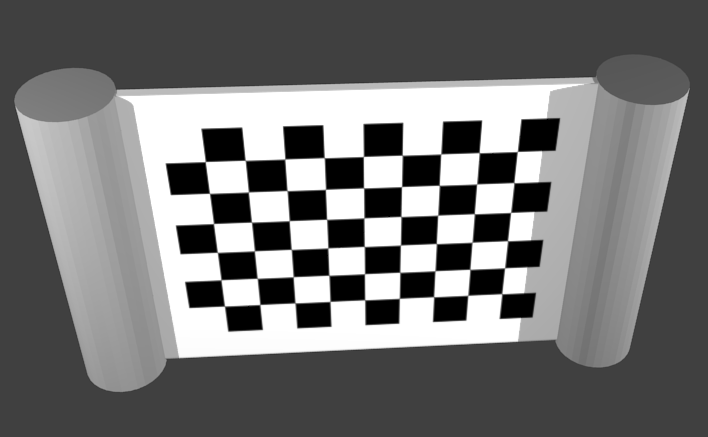
\includegraphics[width=0.5\textwidth]{images/laser_calibration_object}
  \caption{Kalibrierobjekt für die Laserscanner}
  \label{fig:kalibrierobjekt-laser}
\end{figure}

Ein mögliches Kalibrierobjekt ist in \ref{fig:kalibrierobjekt-laser} dargestellt.
Es besteht aus einem Schachbrett, an dessen Rändern Zylinder angebracht sind.
Die Zylinder ergeben im 2D-Schnitt ein Kreissegment, das mithilfe einer 
Hough-Transformation \cite{rohtua} erkannt werden kann. Auf diese Weise können 
auch alle 
auftretenden Geraden erkannt werden. 
Da die Achsen der 
Zylinder des Kalibrierobjekts auf einer Ebene mit der Ebene des Schachbretts liegen, kann die
Position des Kalibrierobjekts aus der Linie die den geringsten Fehler zu den
Mittelpunkten der erkannten Kreise als Teil der Ebene des Kalibrierobjekts
erkannt werden. Die erkannte Position liefert die Orientierung und den Abstand
des Kalibrierobjekts zum Laserscanner. Die Erkennung des Kalibrierobjekts
funktioniert in der Simulation, muss aber noch stabilisiert und mit der
Hardware überprüft werden.

Das Schachbrett am Kalibrierobjekt wird zur Erkennung durch die Kameras benötigt.
Aus der erkannten 6\ac{DOF} Pose der Kameras und der 2\ac{DOF} Pose der Laserscanner 
kann mit mehreren dieser Datensätzen die Position der Laserscanner relativ zu den
Kameras berechnet werden. Die Berechnung kann wie die kinematische Kalibrierung
von einem Optimierer erfolgen. Die Umsetzung des Optimierers steht nach den
Verbesserungen an der Objekterkennung noch aus. 

